%!TEX root = /Users/ede/Documents/Master/19_AS/Ausarbeitung/as-ausarbeitung.tex
\section{Analyse und Klassifikation} % (fold)
\label{sec:analyse_und_klassifikation}

Um die Tag-Rankingverfahren hinsichtlich der oben genannten Anwendungsgebiete zu formulieren und zu optimieren, müssen zunächst die vorhandenen Tags in einer Folksonomy analysiert werden \cite{collectiveKnowledge}. Als Datenbasis aller vorgestellten Ansätze dient die Photocommunity Flickr. Diese Photocommunity Plattform beinhaltet das Konzepts des Tagging und verfügt über eine hohe Anzahl\footnote{Am 12.10.09 erreichte der Bestand von Flickr.com über 4 Milliarden Photos, vgl. http://blog.Flickr.net/en/2009/10/12/4000000000/ } von frei verfügbaren Photos


%TODO: mehr beschreiben, wofür die Analyse und Klassifikation benötigt wird, und was als Ergbenis erwartet wird(z.B. Dass folgende Fragen beantwortet werden)
Damit die Anwendungsgebiete möglichst unterstützen werden können, ist ein genaues Verständnis der Vorgehensweise beim Tagging wichtig. Ebenso ist die Motivation hinter dem Tagging von Bedeutung, also warum Menschen ihre Daten überhaupt annotieren und welches Ziel sie damit verfolgen. Dazu werden mehrere Untersuchungen über eine große Menge von Photos aus Flickr vorgestellt.

Im Folgenden soll kurz auf die Analyse der Tags eingegangen werden, wobei die nachstehenden Fragen beantwortet werden sollen:
\begin{itemize}
	\item     Welche Tags sind vorhanden? Frequenz der Tags?
	\item     Wie gehen Benutzer beim Taggen vor?
	\item     Warum taggen Benutzer?
	\item     In welcher Reihenfolge liegen die Tags vor?
  \item     Anzahl der Tags pro Photo?
	\item     In welchen Beziehungen stehen die Tags untereinander?
	\item     In wie weit gleicht der Inhalt der Photos, wenn gleiche Tags vorhanden sind?
	\item     Können die Tags in Kategorien zusammengefasst werden?
\end{itemize}

Die nächsten Abschnitte beschreiben also zunächst die in Flickr vorhandenen Photos sowie die zugehörigen Tags und klassifizieren diese anschließend, um sie für die Tag Ranking Verfahren sowie für die Evaluation der Verfahren nützlich zu machen.

\subsection{Analyse der Tags und Photos} % (fold)
\label{sub:analyse_der_tags}

\cite{collectiveKnowledge} verwenden über 52 Millionen Photos aus den Jahren 2004 bis 2007 für ihre Untersuchung. Die vorgenommene Auswahl verfügt über 188 Millionen Tags, wovon 3,7 Millionen eindeutig sind. Dies ist also eine statistisch ausreichende Menge, um auf die Gesamtheit schließen zu können.

\begin{figure}[htbp]
    \centering
      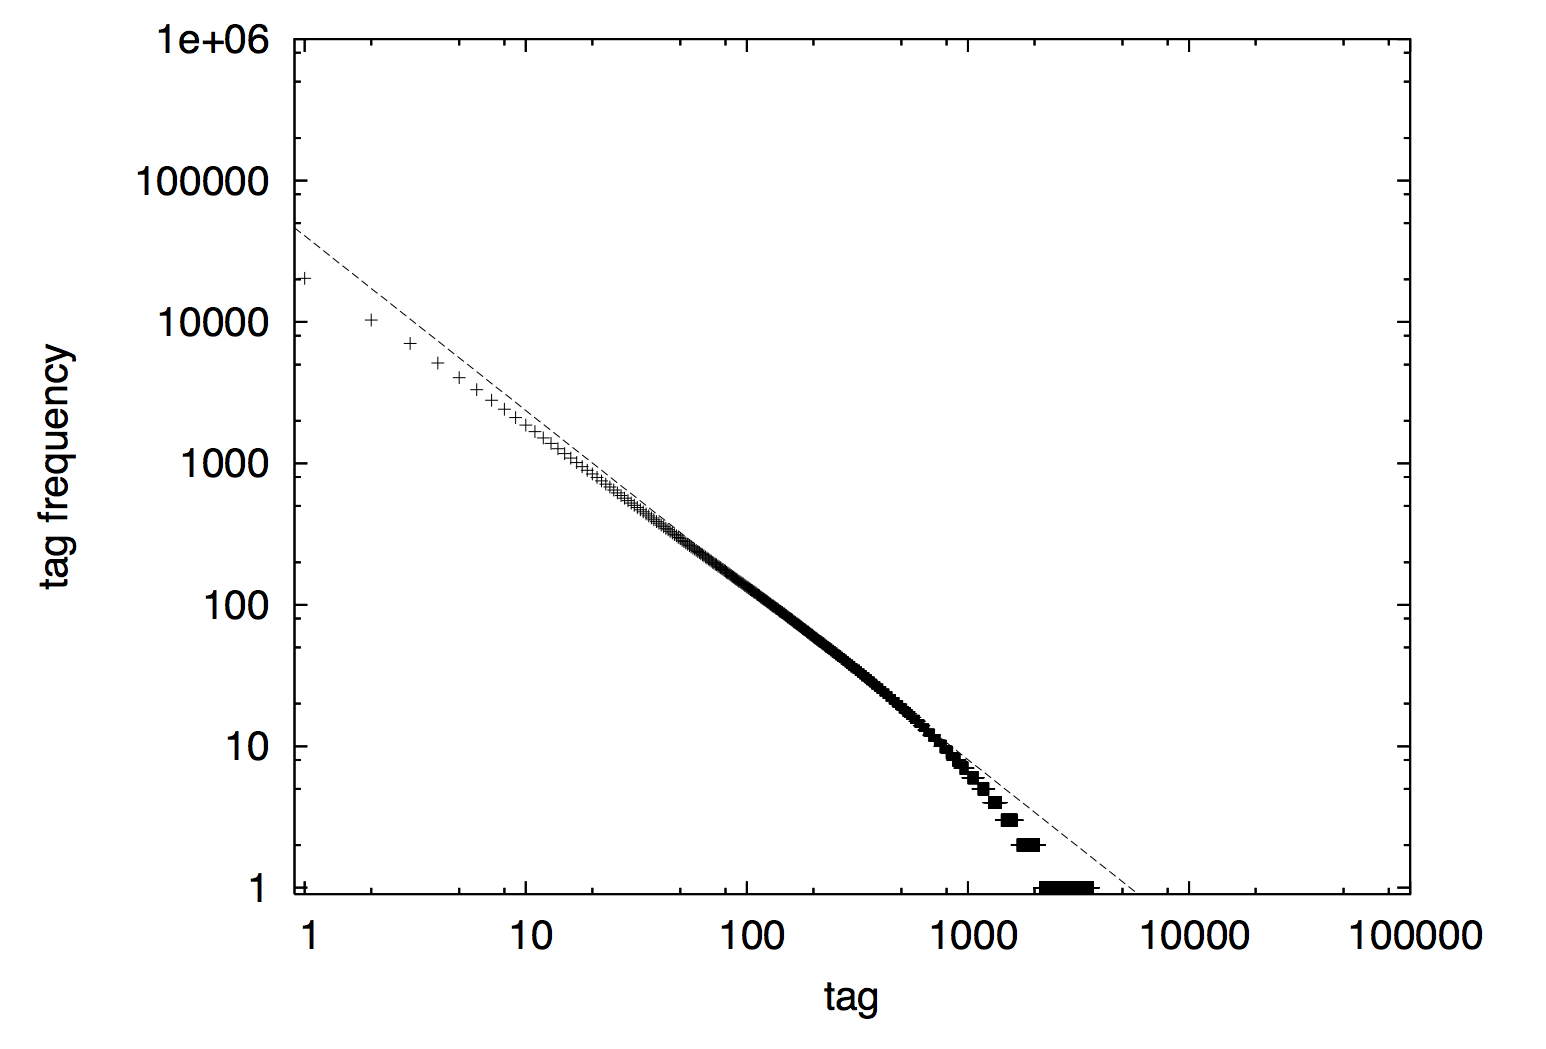
\includegraphics[height=2in]{images/collectiveKnowledge_tag_frequency.png}
    \caption{Häufigkeitsverteilung von 3,7 Millionen eindeutigen Tags in Flickr aus \cite{collectiveKnowledge}. Die Achsen sind hierbei logarithmisch skaliert.}
    \label{fig:images_collectiveKnowledge_word_net_categories}
\end{figure}

Abbildung \ref{fig:images_collectiveKnowledge_word_net_categories} veranschaulicht die Häufigkeitsverteilung der Tags. Die Abszisse repräsentiert die 3,7 Millionen eindeutigen Tags sortiert nach absteigender Häufigkeit, während die Ordinate die Häufigkeit selbst darstellt. Die ablesbare Kurve wird sehr gut durch das Potenzgesetz  beschrieben, vgl. \cite{hpParetoPowerLaw}. Dieses besagt für beobachtete Phänomene in der Welt, dass geringe Vorkommnisse sehr häufig und große Anhäufungen sehr selten auftreten. Im vorliegenden Fall werden einige wenige Tags sehr oft von den Benutzer für Annotationen verwendet, wohingegen die meisten Tags nur selten eingesetzt werden.

In Anbetracht der Aufgabe, dem Benutzer passende Tags für die Annotation vorzuschlagen, ist es laut \cite{collectiveKnowledge} nicht sinnvoll die häufigsten Tags anzubieten, da diese zu allgemein in ihrer Bedeutung sind. So sind die fünf am meisten verwendeten Tags \emph{2006, 2005, wedding, party} und \emph{2004}. Analog dazu sind die extrem selten verwendeten Tags zu spezifisch und eigenen sich ebenfalls nur bedingt für die vorgesehene Aufgabe. Diese Verwendungshäufigkeit von Tags fließt in das Verfahren zum Vorschlagen von Tags nach \cite{collectiveKnowledge} ein und wird in Kapitel \ref{sec:tag_ranking_verfahren} erläutert.

Zu einem ähnlichen Ergebnis gelangen auch \cite{learningToTag} in ihrer Untersuchung von über 640 Millionen Photos aus Flickr, welche in Abbildung \ref{fig:images_learning_to_tag_frequency} veranschaulicht wird. Diese Sammlung enthält insgesamt 1,3 Milliarden Tags, wobei die Autoren eine Unterteilung bezüglich der Art der Tags vornehmen. Ein Prozent der Tags werden mehr als 20.000 Mal verwendet, womit diese laut den Autoren nur wenig Information enthalten. Knapp 6\% der Tags werden als populär angesehen, da sie mehr als 5000 Mal in der Sammlung auftauchen. 33,21 Prozent treten zwischen 50 und 5.000 Mal auf und werden zu den spezifischen Tags gezählt. Alle weiteren, seltener auftretenden Tags, die ca. 60 Prozent der Gesamtmenge ausmachen, gelten als Rauschen, das sie meist falsch geschrieben oder einfach nur irreführend sind.

\begin{figure}[htbp]
    \centering
      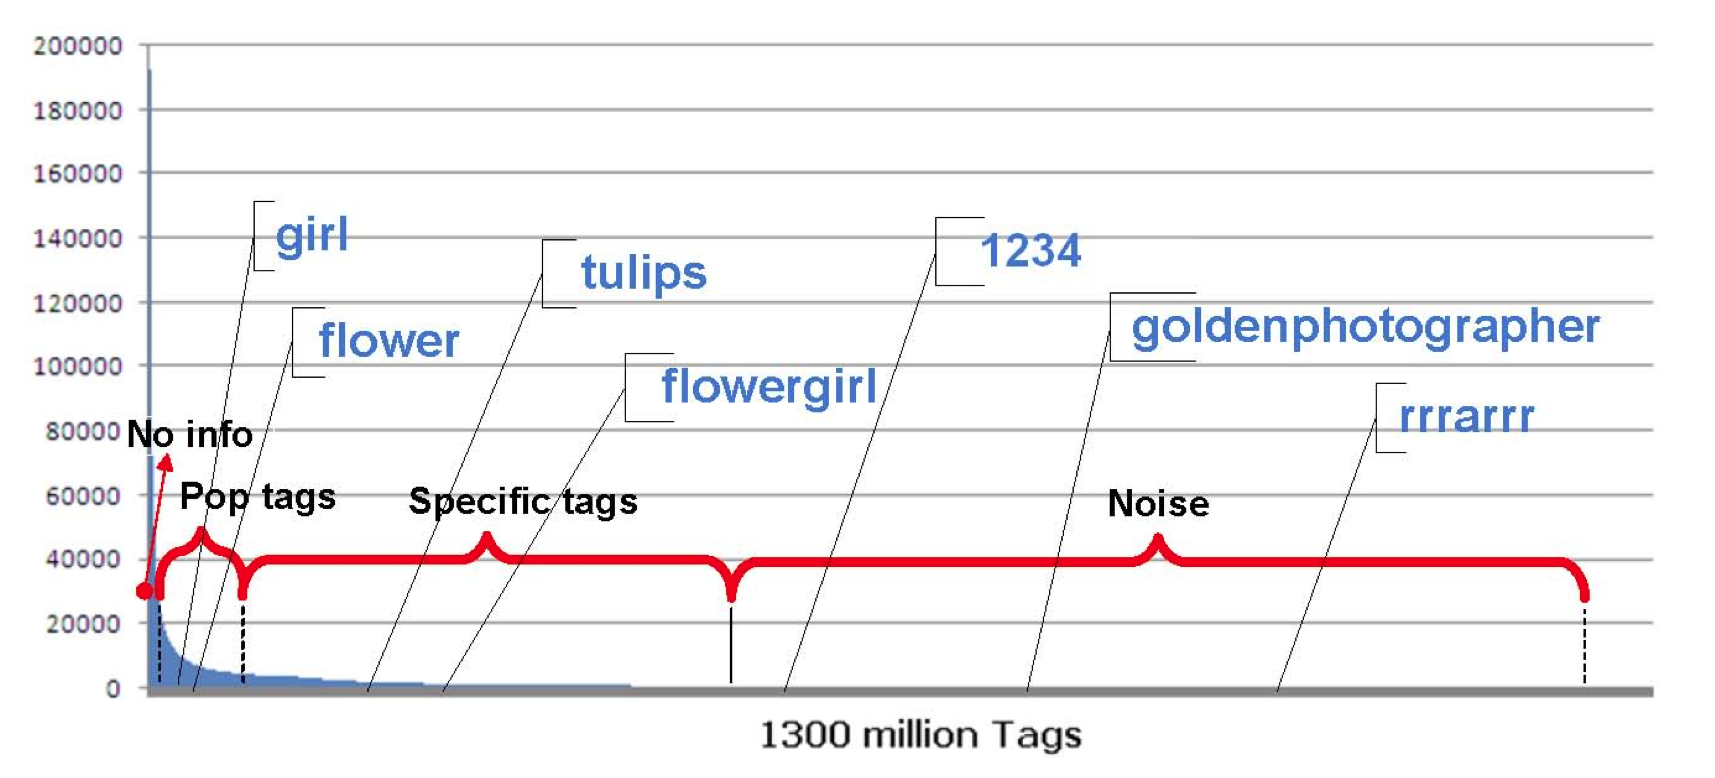
\includegraphics[height=2in]{images/learning_to_tag_frequency.png}
    \caption{Tag Verteilung von über 640 Million Photos aus der Analyse von \cite{learningToTag}, die insgesamt 1,3 Milliarden Tags enthalten.}
    \label{fig:images_learning_to_tag_frequency}
\end{figure}


Bei der Betrachtung der Anzahl der Tags pro Photo zeigt sich ebenfalls eine Verteilung nach dem Potenzgesetz. Laut der Analyse von \cite{collectiveKnowledge} besitzen einige Photos mehr als 50 Tags, der Großteil der Photos mit 64 Prozent Anteil weisen jedoch nur 1 bis 3 Tags auf. Diese Menge eignet sich damit besonders für das Vorschlagen von Tags und zeigt gleichzeitig das Bedürfnis für solche Verfahren.

Jedes Photos in Flickr kann beliebig viele Tags enthalten, wobei diese in der Reihenfolge vorliegen in der sie auch zu dem Photo hinzugefügt wurden. Die Reihenfolge der vergebenen Tags steht dabei in keiner Beziehung zu der Relevanz für das assoziierte Photo. \cite{ranking} untersuchten dazu 1.200 zufällig ausgewählte Photos mit mindestens 10 Tags pro Photo und ließen die Relevanz der Tags für das jeweilige Photo von fünf Probanden bewerten. Nur ein Zehntel der Photos hatte den relevantesten Tag an erster Stelle. Abbildung \ref{fig:images_tag_ranking_psotion_relevant_tag} zeigt die Ergebnisse des Tests mit den Probanden.

\begin{figure}[htbp]
  \centering
    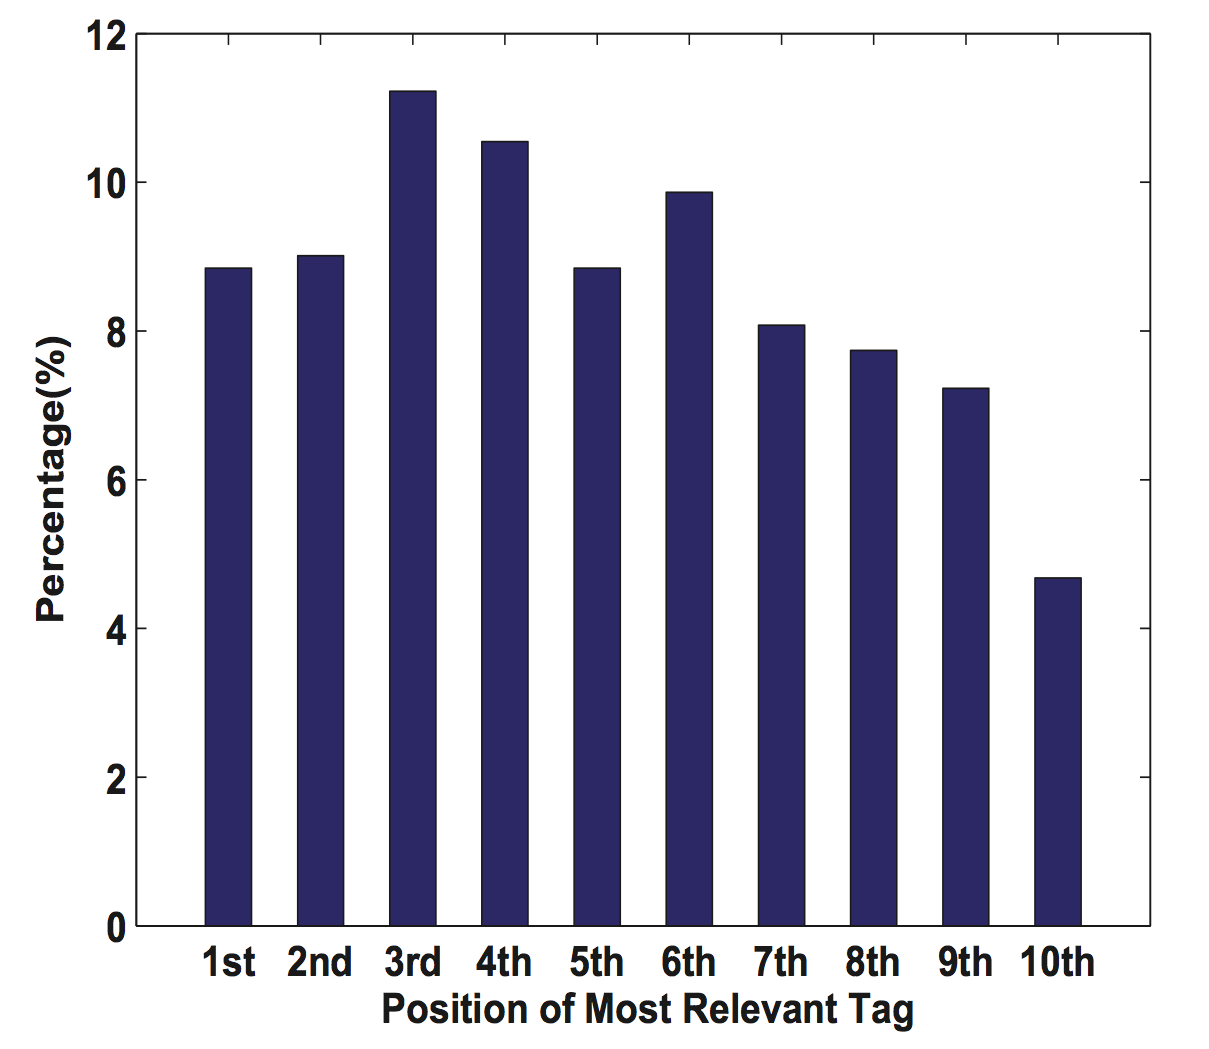
\includegraphics[height=2in]{images/tag_ranking_psotion_relevant_tag.png}
  \caption{Prozentuale Anteile der Photos, die den relevantesten Tag an der n-ten Position der Tag Liste haben. Aus \cite{ranking}}
  \label{fig:images_tag_ranking_psotion_relevant_tag}
\end{figure}
  
Es ist also nicht möglich die Relevanz aus der von Flickr gegebenen Position zu bestimmen. Auffällig ist, dass 70 Prozent aller Photos den relevantesten Tag innerhalb der ersten 10 Positionen haben. Es scheint also ein Zusammenhang zwischen der Eingabesequenz der Tags für ein Photo und der Relevanz des Tags für das Photo zu bestehen, wobei dieser relativ schwach ausgeprägt ist und nicht als qualitative Informationsquelle dienen kann. 

% subsection analyse_der_tags (end)

\subsection{Klassifikation von Tags und Photos} % (fold)
\label{sub:klassifikation_von_tags}

\cite{collectiveKnowledge} untersuchten 52 Millionen Photos und deren Tags aus Flickr. Für die Photos wurde eine Klassifizierung nach der Anzahl gesetzter Tags gewählt. Diese Klassen finden später noch in der Evaluation der Leistung des verwendeten Verfahrens Einsatz. Die Autoren unterteilen die Photos in mehrere Klassen, um das Verhalten des Tag Ranking Verfahrens für Photos mit unterschiedlichem Informationsgehalt der Tags zu analysieren.

\begin{table}[htbp]
\centering
\begin{tabular}{|c|c|c|} 
\hline
 & Tags pro Photo & Anzahl der Photos pro Klasse\\
\hline
Klasse I & 1 & ca. 15,5 Millionen\\
\hline
Klasse II & 2 - 3 & ca. 17,5 Millionen\\
\hline
Klasse III & 4 - 6 & ca. 12 Millionen\\
\hline
Klasse IV & > 6 & ca. 7 Millionen\\
\hline
\end{tabular}
\caption{Definition der Photo-Tag Klassen und die Anzahl der Photos pro Klasse aus \cite{collectiveKnowledge}}
\label{tab:classes_for_tags_collective}
\end{table}





\subsubsection*{Tags} % (fold)
\label{ssub:tags}


Um besser zu verstehen welche Art von Tags die Benutzer vergeben und welche Motive sie taggen, wird in \cite{collectiveKnowledge} eine Abbildung auf die Kategorien aus WordNet\footnote{``Das WordNet ist ein seit 1985 am Cognitive Science Laboratory der Princeton University entwickelter Wortschatz der englischen Sprache.'' aus Wikipedia, abgerufen am 13.12.09.} vorgenommen. Das Ergebnis ist in Abbildung \ref{fig:collectiveKnowledge_word_net_categories} dargestellt.

\begin{figure}[htbp]
  \centering
    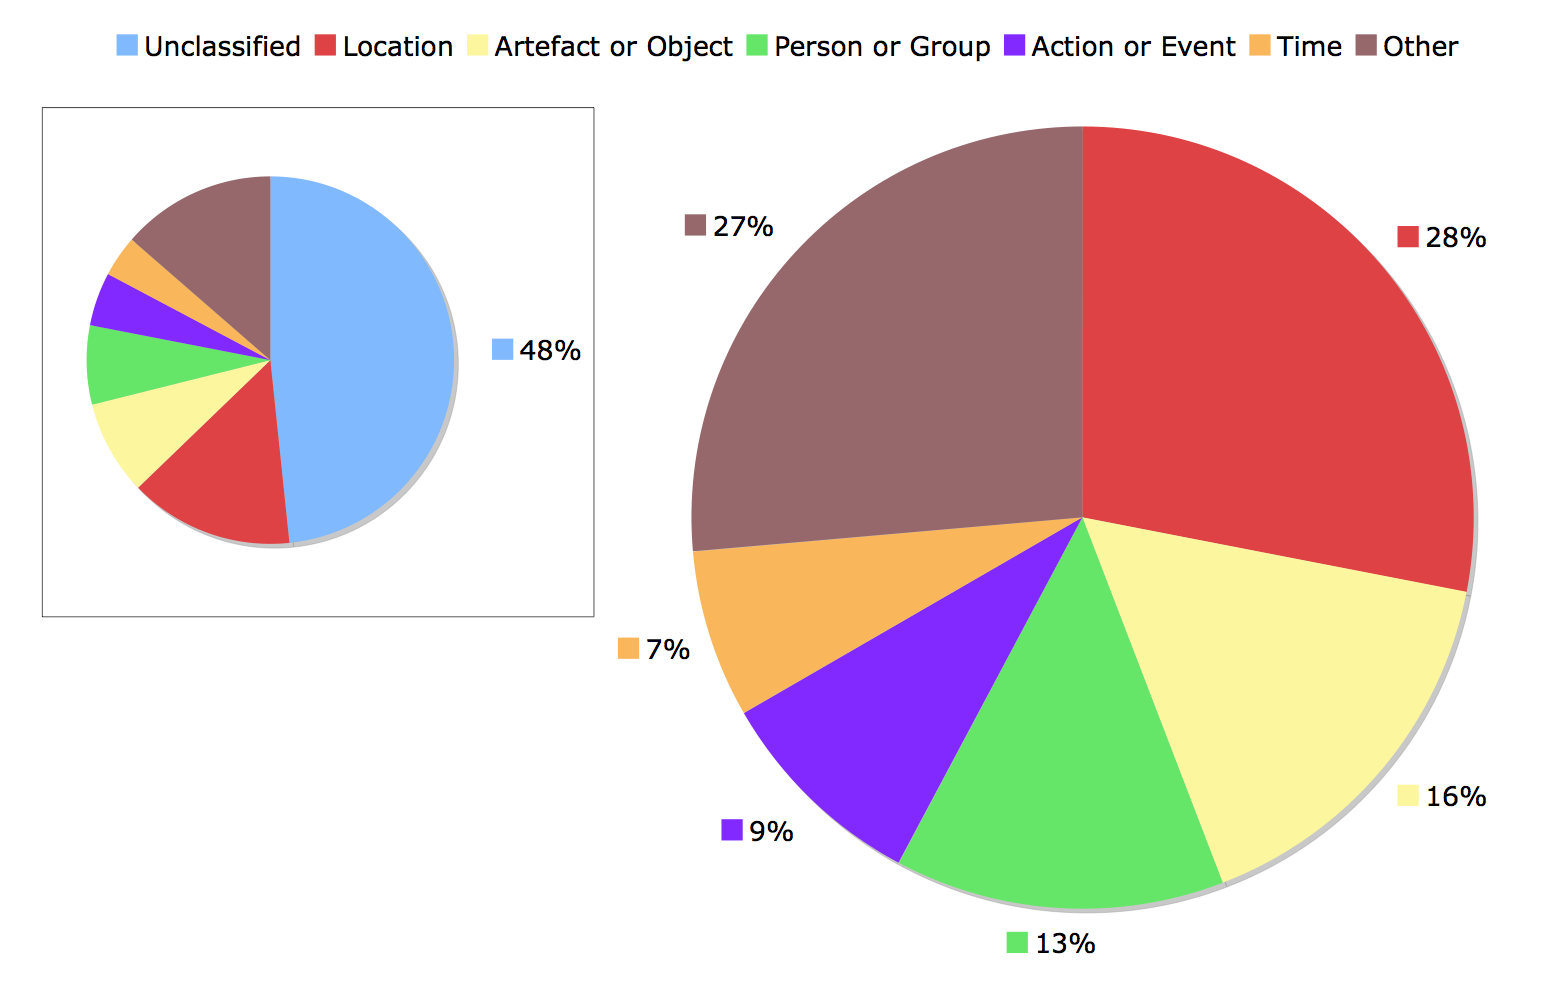
\includegraphics[height=2.5in]{images/collectiveKnowledge_word_net_categories.png}
  \caption{Die häufigsten Kategorien aus WordNet für Flickr Tags nach \cite{collectiveKnowledge}. Das kleine Diagramm zeigt die gesamte Verteilung der WordNet Ergebnisse inklusive der nicht klassifizierten Tags.}
  \label{fig:collectiveKnowledge_word_net_categories}
\end{figure}

52 Prozent der Tags konnten zu WordNet Kategorien zugeordnet werden, die restlichen Tags sind nicht klassifizierbar, das heißt die Begriffe sind nicht im WordNet Katalog enthalten. Dabei wurde, falls mehrere Kategorien für ein Tag in Frage kamen, die als wichtiger eingestufte Kategorie für die Auswertung gewählt. Mit 28 Prozent der klassifizierten Tags erreichen \emph{Ortsangaben} den höchsten Anteil. Weitere Kategorien sind \emph{Menschen oder Gruppen}, \emph{Handlungen oder Ereignisse} und \emph{Zeit}. \cite{collectiveKnowledge} schließen daraus, dass Benutzer nicht nur visuellen Inhalt von Photos, sondern auch Kontextinformationen wie Ort, Zeit und Ereignis annotieren.

Auf Basis dieser Analyse und Klassifikation wurde das Verfahren entwickelt, welches in Abschnitt \ref{sub:ranking_basierend_auf_kollektivem_wissen_nach_zwol} beschrieben wird.

% TODO: Hier noch was mehr zu dem anderen verfahren oder mal was abschließendes und zusammenfassendes

% subsubsection tags (end)  

% subsection klassifikation_von_tags (end)




% section analyse_und_klassifikation (end)
